\chapter{Numerical Integration Methods}
\label{integ}
\graphicspath{{chapter-6/Images/}}

\section{Introduction}
We have been acquainted with the full two-body problem and the restricted full three-body problem and in both cases we have witnessed that the equations of motion are highly complex. An analytical solution for those equations of motion can not be obtained and so to study the dynamical behavior of the binary or the tertiary system, we have to numerically integrate the equations and observe and store the state after each time step. Several methods have been developed for integrating differential equations and most of these methods have been successfully applied to the field of astrodynamics. We will be looking into the basic properties and principles of some important integration methods such as:
\begin{itemize}
\item Runge-Kutta methods - Easy to use and most commonly applied \cite{gillbook}
\item Multistep methods - Offer high accuracy but require storage of previous data points \cite{gillbook}
\item Extrapolation methods - Popular for their extremely high accuracy \cite{gillbook}
\item Taylor Series Method - Popular for high-precision and long-time numerical integration \cite{tsm2011}
\end{itemize}
Every method has its own set of pros and cons and its not easy to pinpoint and select any one integration method. The aim of this chapter will be to present enough details, including the advantages and disadvantages, on each method so that at the end we can make an informed, smart, and logical decision about which integration method will be best suited for our particular application. We will present some general differential equation that will be used as reference for discussing the integration methods. The second-order differential equation expressing the acceleration for an orbiting particle is given as a function of time, position, and velocity as follows \cite{gillbook}:
\begin{equation}
\label{racc}
\ddot{\mathbf{r}} = a(t, \mathbf{r}, \dot{\mathbf{r}})
\end{equation}
%
where $\ddot{\mathbf{r}}$ is the acceleration, $\dot{\mathbf{r}}$ is the velocity, and $\mathbf{r}$ is the position of the orbiting particle. The six dimensional position and velocity vector is given as:
\begin{equation}
\label{state_vec}
\mathbf{y}
=
\begin{bmatrix}
\mathbf{r} \\
\dot{\mathbf{r}}
\end{bmatrix}
\end{equation}
%
Then, the differential equation of motion is given as \cite{gillbook}:
\begin{equation}
\label{diff_eqn}
\dot{\mathbf{y}} = f(t,\mathbf{y}) =
\begin{bmatrix}
\dot{\mathbf{r}} \\
a(t, \mathbf{r}, \dot{\mathbf{r}})
\end{bmatrix}
\end{equation}
%
These general equations will be used when explaining the integration methods in the following sections.

\section{Runge-Kutta Methods}
\label{RK}
Given the initial values $y_0$ at some time $t_0$, we can approximate the value $y$ at some time $t_0 + h$ as follows \cite{gillbook}:
\begin{align}
\label{euler1}
\mathbf{y}(t_0 +h) & \approx \mathbf{y}_0 + h \dot{\mathbf{y}_0}\\
\label{euler2}
& = \mathbf{y}_0 + h f(t_0, \mathbf{y}_0)
\end{align}
%
where $h$ is the \textit{step size}, and the above process is called the \textit{Euler Step}. Using \Cref{euler2}, one can obtain approximate values $\eta_i$ of the solution of the differential equation at specific times $t_i = t_0 + ih$  $\forall \text{ } i = 1,2,3,...$ \cite{gillbook}. The step size should be sufficiently small so that the approximate solution obtained over multiple time steps is still close to the actual solution and does not diverge from it. A better approximating method is given below \cite{gillbook}:
\begin{equation}
\mathbf{y}(t_0 +h) \approx \mathbf{y}_0 + h\phi = \eta(t_0 + h)
\end{equation}
%
where $\eta(t_0 + h)$ is the approximate solution to the differential equation, and $\phi$ is called as the incremental function. In the classical \gls{RK4} method, the incremental function is given as follows \cite{gillbook}:
\begin{equation}
\phi_{RK4} = \frac{1}{6}(\mathbf{k_1} + 2\mathbf{k_2} + 2\mathbf{k_3} + \mathbf{k_4})
\end{equation}
%
where the $\mathbf{k}$ terms are defined as \cite{gillbook}:
\begin{align}
\mathbf{k_1} &= f(t_0, \mathbf{y}_0)\\
\mathbf{k_2} &= f(t_0 + h/2, \mathbf{y}_0 + h\mathbf{k_1}/2)\\
\mathbf{k_3} &= f(t_0 + h/2, \mathbf{y}_0 + h\mathbf{k_2}/2)\\
\mathbf{k_4} &= f(t_0 + h, \mathbf{y}_0 + h\mathbf{k_3})
\end{align}
%
The \gls{RK4} method can approximate the exact solution upto terms of order $h^4$, which means that if one reduces the step size for integration by, say half, then the resulting global error from the numerical integration will reduce by a factor of 16. It also means that the difference between the approximated solution and the exact solution i.e. the local truncation error, will be of the order of $h^5$. In general an \gls{RK} method is said to be of order $p$ if the local truncation error is of order $h^{p+1}$ or if the approximated solution matches the exact solution upto an order of $h^p$ \cite{feagin}. The local truncation error in the \gls{RK4} method is given as follows \cite{gillbook}:
\begin{equation}
\label{rk4_error}
e_{RK4} = |y(t_0 + h) - \eta(t_0 + h)| \leq const.h^5
\end{equation}
%
what we discussed right now was the \gls{RK4} method, as an example, but we can also present a more generalized approach to the (explicit) Runge-Kutta methods.

\subsection{General Runge-Kutta Methods}
The general Runge-Kutta method consists of two tasks: the first one is to compute the $s-stage$ values which are needed for forming the incremental function $\phi$, and the second part is to finally compute the approximated solution of the differential equation at a given time $t_n$. So, for an \textit{s-stage} \gls{RK} method, the follwing $s$ function evaluations:
\begin{align}
k_1 &= f(t_0 + c_1h, y_0) \\
k_i &= f(t_0 + c_ih, y_0 + h \sum_{j=1}^{i-1}a_{ij}k_j) \text{ } \forall \text{ } i = 2, 3, ...s
\end{align}
%
are utilized in creating the increment function $\phi$ as follows \cite{gillbook}:
\begin{equation}
\label{phi_general}
\phi = \sum_{i=1}^{s} b_ik_i
\end{equation}
%
from which the approximate solution is obtained as:
\begin{equation}
\eta(t_0 + h) = y_0 + h\phi
\end{equation}
%
The coefficients $c_i$, $b_i$, and $a_{ij}$ are usually presented in a tabular form, called the \textit{Butcher's Tableau}, as shown in \Cref{fig:rk_tab} \cite{gillbook}.
%
\begin{figure}[h]
\centering
\captionsetup{justification=centering}
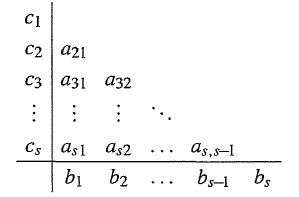
\includegraphics[scale=1]{rk_tab.png}
\caption{The Butcher's Tableau depicting the coefficients used in the \gls{RK} methods \cite{gillbook}.}
\label{fig:rk_tab}
\end{figure}
%\FloatBarrier
%
These coefficients are chosen such that they maximize the order $p$ of the local truncation error. They are determined in a manner such that they satisfy the following relations \cite{gillbook}:
\begin{align}
\sum_{i=1}^{s} b_i &= 1\\
c_1 &= 0 \\
c_i &= \sum_{j=1}^{i-1}a_{ij} \text{   } (i>1)
\end{align}
%
For higher-order \gls{RK} methods, specifically the $6^{th}$ and the $8^{th}$ order, the coefficients are presented in the appendix of \cite{jstor} in the form of the \textit{Butcher's Tableau}.

\subsection{Embedded Runge-Kutta Methods}
It is possible to develop \gls{RK} methods of neighboring orders that are based on the same set of $s$ function evaluations. This is called as \textit{embedded} \gls{RK} method. What we do in this method is that we evaluate the regular \gls{RK} method but independently for two different yet nearby orders, say for example orders 10 and 8, and then we get two independent estimates of the solution of the differential equation from which we try to estimate the local truncation error. This method allows a very easy estimation of the local truncation error which is utilized in efficient stepsize control (discussed later) during the integration process.

An s-stage embedded \gls{RK} method will yield two independent approximations of the exact solution and these are expressed as follows \cite{gillbook}:
\begin{align}
\eta(t_0+h) &= y_0 + h\sum_{i=1}^{s} b_ik_i\\
\hat{\eta}(t_0+h) &= y_0 + h\sum_{i=1}^{s} \hat{b}_ik_i
\end{align}
%
with orders $p$ and$p+1$ respectively, with local truncation error given as follows \cite{gillbook}:
\begin{align}
e &= |y(t_0 + h) - \eta(t_0 + h)| \leq const.h^{p+1} \\
\hat{e} &= |y(t_0 + h) - \hat{\eta}(t_0 + h)| \leq const.h^{p+2}
\end{align}
%
we can see from the above equation that $\hat{e}$ is smaller than $e$ by an order of $h$, this allows us to make the following approximation \cite{gillbook}:
\begin{equation}
e = |y - \eta| \approx |\hat{\eta} - \eta|
\end{equation}
%
which basically indicates that we can estimate the local truncation error of the \gls{RK} method of order $p$ just by taking the difference of the two outcomes of the embedded \gls{RK} method. At this point, we should also discuss the embedded \gls{RK} notation, which is usually given in the literature as $RKp(q)-s$, where $RK$ refers to Runge-Kutta, $p$ refers to the actual order of the \gls{RK} method that we intend to use to perform our integration, $q$ refers to the neighboring order of \gls{RK} method that we use as part of the embedded \gls{RK} procedure which is used only to estimate the local truncation error, and finally $s$ represents the number of \textit{s-stage} evaluations involved in both the $p$ and $q$ order \gls{RK} methods \cite{gillbook}. The coefficients for the RK8(7)-13 method, which is considered as a high-order \gls{RK} method, is given in the reference \cite{gillbook} in the \textit{Butcher's Tableau} format.

As stated before, an easy estimation of the local truncation error will help in efficient step size control during the integration process, which is our next topic of discussion.

\subsection{Step Size Control}
In numerical integration, it is desired that every integration step contributes uniformly towards the total integration error. This can be achieved by an approach called the \textit{Step Size Control}. A common method for performing stepsize control is with the embedded \gls{RK} method wherein we can easily estimate the truncation error at each step. The stepsize control method then tries to limit this local truncation error for each step \cite{gillbook}.

Now for a given step size $h$, we perform the integration step using the embedded \gls{RK} method and then the estimated local truncation error is given as \cite{gillbook}:
\begin{equation}
e(h) \approx |\hat{\eta} - \eta|
\end{equation}
%
If the above local truncation error is larger than a given tolerance value $\epsilon$ then the same integration step is repeated but this time with a smaller step size $h^*$. The new local truncation error can then be computed as \cite{gillbook}:
\begin{equation}
e(h^*) = e(h)\left( \frac{h^*}{h} \right)^{p+1}
\end{equation}
%
where $p$ is as defined earlier, the order of the \gls{RK} method. We know that $e(h^*)$ has to be smaller than the specified tolerance $\epsilon$ which means that the maximum allowable value of $e(h^*)$ can be equal to the specified tolerance and no more than that. From this information we can reverse engineer the maximum allowable value for the step size $h^*$ as follows \cite{gillbook}:
\begin{equation}
h^* = \sqrt[p+1]{\frac{\epsilon}{e(h)}} \times h
\end{equation}
%
Using the above step size or a lower value, the integration step is repeated in the scenario when the original step size $h$ results in a local truncation error greater than a specified tolerance. If the integration step with $h^*$ is successful (ideally it should be since it has been reverse calculated from the tolerance), then the same can be used for the next integration step. However the reader should note that the new step-size value is allowed to differ from the old step-size value only by a factor of 2 to 5 and no more than that to avoid rapid oscillations in step-size change. This whole process of step-size control continues for every integration step to ensure uniformity in individual local truncation errors. This process can be automated in a computer code but to initiate the process, the user obviously has to provide an initial guess for the starting step size \cite{gillbook}.

\subsection{Runge-Kutta-Nystr\"om Methods}
\gls{RKN} methods have been developed especially for second-order differential equations, the kind we usually deal with in astrodynamics. The approach involves converting the second-order differential equation of the form given by \Cref{racc} into a system of first-order differential equations and then perform the standard \gls{RK} method over it. Doing this, one arrives at the following solution \cite{gillbook}:
\begin{equation}
\label{rkn1}
\begin{aligned}
\mathbf{r}(t_0+h) &= \mathbf{r}_0 + h\mathbf{v}_0 + h^2 \sum_i \bar{b}_i k_i^* \\
\mathbf{v}(t_0+h) &= \mathbf{v}_0 + h\sum_i b_i k_i^*
\end{aligned}
\end{equation}
%
where $r$ represents the position vector, $v$ represents the velocity vector and is equal to $\dot{r}$ from \Cref{racc}, $r_0$ and $v_0$ are the initial position and velocity, $h$ is the step size. The term $k_i^*$ is defined as follows \cite{gillbook}:
\begin{equation}
k_i^* = a\left( t_0 + c_ih, \mathbf{r}_0 + c_ih\mathbf{v}_0 + h^2 \sum_j \bar{a}_{ij} k_j^*, \mathbf{v}_0+h\sum_j a_{ij} k_j^*  \right)
\end{equation}
%
where the coefficients are defined as follows \cite{gillbook}:
\begin{equation}
\label{rkn_coeff}
\begin{aligned}
\bar{a}_{ij} &= \sum_K a_{iK} a_{Kj} \\
\bar{b}_i &= \sum_j b_j a_{ji}
\end{aligned}
\end{equation}
%
Apparently, the advantages of the \gls{RKN} method over the standard \gls{RK} method is seen only when the second-order differential equation does not have any dependence on the velocity or the first derivative term on the right-hand side of \Cref{racc} \cite{gillbook}. We have seen from the equations of motion of the full two-body problem and restricted full three-body problem that the acceleration term always has explicit dependence on the velocity term. So an early conclusion regarding only the \gls{RKN} method can be made that since it does not offer any advantage over the regular \gls{RK} method, it shall not be used for the future thesis work.

\section{Multistep Methods}
So far what we discussed, the Runge-Kutta methods, can be classified as single-step methods since all individual integration steps are independent of each other. The $s-stage$ function evaluations do not depend on the values that were computed in the previous integration steps. Thus, this method requires no storage of values from previous integration steps and in a way helps in reducing loads on the computer memory for a simulator. But in a way one can also say that all those computed values are being 'wasted' and that they can be utilized for future integration step computations. This is where the Multistep Method comes into the picture. This category of numerical integrators require storage of previous step values as they are utilized in future computations. We will begin with a brief introduction to the core principles of multistep integration methods.

We will consider the differential equation of the form $\dot{y} = f(t,y)$. It is assumed that we already have some initial approximate solutions to the differential equation, let's call these solutions $\eta_j$, at equidistant time values say $t_j = t_0 + jh$ where $j = 0,1,2,...i$. Now consider a polynomial $p(t)$ that interpolates some values $f_j = f(t_j, \eta_j)$ at previous times $t_j$ for which we already have the approximate solutions $\eta_j$. Now we already have approximate solutions until the time value $t_i$ as we said earlier, but we need to perform the integration step to get the approximate solution for the next time step i.e. at $t = t_i + h$. This is shown in the form of an equation as follows \cite{gillbook}:
\begin{equation}
\eta_{i+1} = \eta_i + \int_{t_i}^{t_i + h} p(t) dt = \eta_{i+1} = \eta_i + h \phi
\end{equation}
%
where $\phi$ is the incremental function. So from this we can get the following result \cite{gillbook}:
\begin{equation}
\phi = \frac{1}{h} \int_{t_i}^{t_i + h} p(t) dt
\end{equation}
%
This forms the basis of the multistep method. We see that we need previous function evaluations $f_j$ from previous time steps and use it to create an interpolating polynomial which is then utilized to create the incremental function $\phi$ that is ultimately utilized in performing the next integration step. The initial values to start a multistep method integration process can be obtained by using a high-order standard Runge-Kutta method i.e. get the function values, store them and then use them for future multistep integration steps.

\subsection{Adams-Bashforth Methods}
In this subsection we will utilize the introductory ideas presented earlier and present a multistep integration method called as the \gls{AB} method. Now consider that we already have certain $m$ data points, which are basically previous time steps and the corresponding function values, given as follows \cite{gillbook}:
\begin{equation}
(t_{i-m+1}, f_{i-m+1}),...,(t_i, f_i)
\end{equation}
%
So the values in the bracket above are already known. Now what we do is, we create an interpolating polynomial based on these known data points, let's call this polynomial as $p_m^i(t)$ and it is given as follows \cite{gillbook}:
\begin{equation}
\label{inter_poly}
p_m^i(t) = \sum_{j=0}^{m-1} (-1)^j
\begin{bmatrix}
-\sigma \\
j
\end{bmatrix}
\triangledown^j f_i
\end{equation}
%
where
\begin{equation}
\label{bin_coef}
\begin{bmatrix}
-\sigma\\
j
\end{bmatrix}
= \frac{(-\sigma)(-\sigma-1)...(-\sigma-j+1)}{j!}
\end{equation}
%
is called the binomial coefficient. The term $\triangledown^j f_i$ calculates the backward-differences of the known function values $f$ as follows \cite{gillbook}:
\begin{equation}
\label{f_ab}
\begin{aligned}
\triangledown^0 f_i &= f_i \\
\triangledown^1 f_i &= f_i - f_{i-1} \\
\triangledown^n f_i &= \triangledown^{n-1} f_i - \triangledown^{n-1} f_{i-1}
\end{aligned}
\end{equation}
%
Using these newly defined expressions and notations, we can finally design the increment function $\phi$ for an $m$ order \gls{AB} method integrator as follows \cite{gillbook}:
\begin{equation}
\label{phi_ab}
\phi_{ABm} = \frac{1}{h} \int_{t_i}^{t_i + h} p_m^i(t)dt = \sum_{j=0}^{m-1} \gamma_j \triangledown^j f_i
\end{equation}
%
where the coefficient $\gamma$ is computed from a recurrence relation \cite{gillbook}:
\begin{equation}
\label{gamma_ab}
\gamma_j = 1 - \sum_{k=0}^{j-1} \frac{1}{j+1-k} \gamma_k
\end{equation}
%
The starting value of $\gamma$ can be taken as 1. Thus by using \Cref{f_ab}, \Cref{phi_ab} and \Cref{gamma_ab}, we can finally compute the solution of the differential equation for the next time step as follows:
\begin{equation}
\label{ab_step}
\eta_{i+1} = \eta_i + h\phi
\end{equation}
%
The reader should note that $\eta_i$ is already known, $h$ is the step size, and $\phi$ is obtained using \Cref{f_ab}, \Cref{phi_ab} and \Cref{gamma_ab}. The local truncation error for the \gls{AB} method is computed as \cite{gillbook}:
\begin{equation}
\label{eab}
e_{ABm} \approx h^{m+1} |\gamma_m f_i^{(m)}|
\end{equation}
%
where $f_i^{(m)}$ is the $m^{th}$ derivative of $f$ which is computed using \Cref{f_ab}. The approach we presented utilizes the backward-differences of the function $f_i$ but there is another approach listed in \cite{gillbook}, which avoids computing the backward-differences, that can also be used which is more convenient and efficient to use. As per this method the increment function can be written only in terms of the function values $f_j$ as follows:
\begin{equation}
\label{phi_ab_2}
\phi_{ABm} = \sum_{j=1}^m \beta_{mj} f_{i-m+j}
\end{equation}
%
where the coefficients $\beta$ are calculated as follows:
\begin{equation}
\label{beta_ab}
\beta_{mj} = (-1)^{m-j} \sum_{l=m-j}^{m-1} \gamma_l
\begin{bmatrix}
l\\
m-j
\end{bmatrix}
\text{  } \forall j=1,...,m
\end{equation}
%
where the binomial coefficient is calculated in the same way as that in \Cref{bin_coef}. This approach does not allow easy local error-estimation and change of order between subsequent integration steps, unlike the backward-difference approach.

\subsection{Adams-Moulton and Predictor-Corrector Methods}
In the previous multistep method, \gls{AB} method, the polynomial $p(t)$ was defined using the function values upto and including $f_i$ at time $t_i$ but the integration was performed for the next time step i.e. from $t_i$ to $t_{i+1}$. Another multistep method called the \gls{AB} method constructs the polynomial $p(t)$ using the function value upto and including $f_{i+1}$ at time $t_{i+1}$ thus making the integrated solution more accurate than the \gls{AB} method. The polynomial for this \gls{AM} method is given as \cite{gillbook}:
\begin{equation}
\label{poly_am}
p_m^{i+1}(t) = \sum_{j=0}^{m-1} (-1)^j
\begin{bmatrix}
-\sigma+1 \\
j
\end{bmatrix}
\triangledown^j f_{i+1}
\end{equation}
%
where all terms are computed in the same manner as explained for \Cref{inter_poly}. The incremental function is given as \cite{gillbook}:
\begin{equation}
\label{phi_am}
\phi_{AMm} = \sum_{j=0}^{m-1} \gamma_j^* \triangledown^j f_{i+1}
\end{equation}
%
where the coefficient $\gamma_j^*$ can be evaluated using the recurrence relation \cite{gillbook}:
\begin{equation}
\label{gamma_am}
\gamma_j^* = -\sum_{k=0}^{j-1} \frac{1}{j+1-k} \gamma_k^*
\end{equation}
%
Like before, the starting $\gamma$ value can be taken as 1. The local truncation error for the \gls{AM} method is given as \cite{gillbook}:
\begin{equation}
e_{AMm} \approx h^{m+1} |\gamma_m^* f_i^{(m+1)}|
\end{equation}
%
For the same order of integrator, $m$, the \gls{AM} method has a smaller error per step than the \gls{AB} method since the error constant $\gamma_m^*$ is smaller than $\gamma_m$ \cite{gillbook}. Just like the \gls{AB} method, the \gls{AM} method can also be designed without having to use the backward-differences of $f_j$ function values and so the new increment function is defined as follows \cite{gillbook}:
\begin{equation}
\label{phi_am_2}
\phi_{AMm} = \sum_{j=1}^m \beta_{mj}^* f{i+1-m+j}
\end{equation}
%
where the coefficient is defined as \cite{gillbook}:
\begin{equation}
\label{beta_ab}
\beta_{mj}^* = (-1)^{m-j} \sum_{l=m-j}^{m-1} \gamma_l^*
\begin{bmatrix}
l\\
m-j
\end{bmatrix}
\text{  } \forall j=1,...,m
\end{equation}
%
Computing the next integration step is not that direct in case of the \gls{AM} method as compared to the \gls{AB} method because the increment function evaluation depends on a future function evaluation $f_{i+1}$ at time $t_{i+1}$ and so we can not simply use the relation like the one given in \Cref{ab_step} to perform the integration. The way this works is, that one has to combine an order $m$ \gls{AB} method with an order $m$ or $m+1$ \gls{AM} method in a so-called \gls{PECE} algorithm to get the solution $\eta_{i+1}$ for the differential equation. The algorithm is listed as follows \cite{gillbook}:
\begin{itemize}
\item Calculate the initial estimate of the solution to the differential equation at time $t_{i+1}$ using the \gls{AB} method.
\item Using the estimated solution previously computed, the function value $f_{i+1}$ at time $t_{i+1}$ is calculated.
\item Using the function value previously computed, the new incremental function for the \gls{AM} method is calculated and through it the new estimate of the solution to the differential equation is calculated.
\item Using the new estimate of the solution, the function value $f_{i+1}$ is recomputed which will be utilized in the next integration step.
\end{itemize}
%
In principle, the last two steps mentioned in the algorithm above have to be repeated until convergence is achieved for the \gls{AM} method but doing so will result in repeated evaluation of the function value $f_{i+1}$ and then recomputation of the incremental function $\phi$. This will demand considerable computational effort, but \cite{gillbook} mentions that the \gls{PECE} algorithm can be implemented if one can accept slightly higher local truncation error. A relative value for this error is not easy to provide since it depends on how many iterations one performs to get the best estimate of the solution. If computational resources can be increased, then performing multiple iterations of the final two steps in the algorithm should be feasible.

The reader should note that when it comes to multistep integration methods, stability becomes an issue when we are using high-order integrators. One has to be careful with the selected step size because even if the local truncation error is small, the global integration error can increase exponentially if the appropriate stepsize for higher-order multistep methods is not chosen. This is not an issue with lower-order integrators even if a relatively large step size is used for them. Using the \gls{PECE} algorithm improves the stability of the multistep integration method considerably \cite{gillbook}. \Cref{fig:multi} depicts what we just discussed, as one can see, the \gls{AB} method of order 8 becomes highly unstable relative to its lower-order couterpart. The combined \gls{AB} and \gls{AM} method as discussed in the \gls{PECE} algorithm, denoted in the graphs as 'ABM8', offers lowest global errors and remains highly stable over the course of integration even with twice the step size as that for the other two methods depicted in the graph \cite{gillbook}. Clearly, we have a winner in this scenario.
%
\begin{figure}[h]
\centering
\captionsetup{justification=centering}
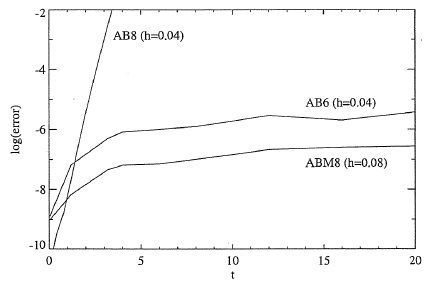
\includegraphics[scale=1]{multi.png}
\caption{Global integration error versus time for different multistep methods and their order. ABM refers to the Adams-Bashforth-Moulton method which is basically the \gls{PECE} algorithm. \cite{gillbook}.}
\label{fig:multi}
\end{figure}
\FloatBarrier
%
Since we will be working with perturbing accelerations as well in our simulations, \cite{gillbook} suggests that only the central gravitational field acceleration term should be updated with the new coordinates obtained from the third step (corrector step) of the \gls{PECE} algorithm and the perturbing acceleration should be updated with the output of coordinates from the first step (predictor step) of the \gls{PECE} algorithm only. This increases the stability of the integrator when one is dealing with orbital perturbations in their simulators. \cite{gillbook} also recommends that for the purpose of orbit simulations, one should use multiistep methods of orders in the range of 8 to 12.

\subsection{Variable-Order and Variable Step Size Methods}
The Adam methods that we have discussed so far, perform integration with a constant step size, but in some cases, one may have to change the step size in between the integration to reduce the local errors so that the integrator remains stable and the global errors do not increase exponentially. For arbitrary step sizes the $m^{th}$-order predictor formula (\gls{AB} method) for the computation of the estimated solution at the next time step i.e. $t_{i+1}$ can be written as \cite{gillbook}:
\begin{equation}
\label{var1}
\eta_{i+1} = \eta_i + (t_{i+1} - t_i) \sum_{j=0}^{m-1}g_j(i) \phi_j(i)
\end{equation}
%
where the coefficients are defined as follows \cite{gillbook}:
\begin{equation}
\label{varg}
g_j(i) = \frac{1}{t_{i+1} - t_i} \int_{t_i}^{t_{i+1}} \prod_{l=0}^{j-1} \frac{t-t{i-l}}{t_{i+1} - t_{i-l}} dt
\end{equation}
%
\begin{equation}
\label{varphi}
\phi_j(i) = \prod_{l=0}^{j-1}(t_{i+1} - t_{i-l}) f[t_i,...,t_{i-j}]
\end{equation}
%
where the term $f[t_i,...,t_{i-j}]$ is called divided differences and is defined as follows \cite{gillbook}:
\begin{equation}
\begin{aligned}
f[t_i] &= f_i \\
f[t_i, t_{i-1}] &= \frac{f_i - f_{i-1}}{t_i - t_{i-1}} \\
f[t_i, t_{i-1}, t_{i-2}] &= \frac{f[t_i, t_{i-1}] - f[t_{i-1}, t_{i-2}]}{t_i - t_{i-2}}
\end{aligned}
\end{equation}
%
To use the variable-order and stepsize method, the error for the current order and nearby order is calculated for the predictor formula first. A new step size based on the estimated error for the current order and step size is also estimated. The error-estimation formula is given in \Cref{eab}. A stepsize change is performed only if the new step size requires a change from the current one by a factor of 2 or more. The change in order is done by changing the value of $m$ in the predictor formula to $m-1$ or $m+1$.

\section{Extrapolation Methods}
Extrapolation methods are powerful, in the sense that they offer extremely high accuracy in the integration process. These methods are, like their Runge-Kutta counterparts, single step methods.

\subsection{Mid-Point Rule}
Consider the differential equation of the form $\dot{y} = f(t,y)$ with given initial conditions $y(t_0) = y_0$. We want to calculate the solution to the differential equation at some time $t_0+H$. To do this, the time interval $[t_0, t_0 +H]$ is first converted into $n$ number of steps, each of equal size $h = H/n$. For the first time step we obtain an approximation $u_1$ using the simple \textit{Euler Step} through \Cref{euler2} and obtain further approximations $u_i$ using the so-called \textit{mid-point rule}. These are shown as follows \cite{gillbook}:
\begin{equation}
\begin{aligned}
u_1 &= y_0 + h f(t_0, y_0) \\
u_{i+1} &= u_{i-1} + 2h f(t_0+ih, u_i)
\end{aligned}
\end{equation}
%
This gives an approximate solution to the differential equation at time $t_0 + H$ as follows \cite{gillbook}:
\begin{equation}
y(t_0 + H) \approx \eta(h) = \frac{1}{4}u_{n-2} + \frac{1}{2}u_{n-1} + \frac{1}{4}u_n
\end{equation}
%
The error between the exact solution and the approximated solution is an asymptotic expansion in the square of the stepsize $h^2$ and so the error can be reduced drastically by employing small step size.

\subsection{Extrapolation}
The method presented earlier, is of low order and one of the ways to increase the order of integration is by performing the integration step again with a different step size $h*$ all the while keeping the result from the old step size as well. Then we can use the following formula \cite{gillbook}:
\begin{equation}
y(t_0 +H) \approx \eta^* = \frac{h^{*^2}\eta(h) - h^2\eta(h^*)}{h^{*^2} - h^2}
\end{equation}
%
By doing the above process, the error in the integration step is reduced by two orders i.e. reduced by an order of $h^2$. We can use even higher-order extrapolation formulas to further improve the order of integration. This is done by basically performing the same integrations step with several step sizes $h_i = H/n_i$ where $n_i = 2,4,6,8,12,...$. The higher-order extrapolation then takes place as follows \cite{gillbook}:
\begin{equation}
\label{extrapol}
y(t_0 +H) \approx \eta_{i,j+1} = \frac{h_{i-j}^2\eta_{i,j} - h_i^2\eta_{i-1,j}}{h_{i-j}^2 - h_i^2}
\end{equation}
%
The above equation depends on the sequence shown in \Cref{fig:seq}. Each entry in the figure is a combination of the entries to the left and upper left of it and this is exactly what is done in \Cref{extrapol}. Thus to get a high-order estimate to the solution of the differential equation, a given integration step has to be done again and again with different step sizes using the mid point rule so that towards the end and using the sequence given in \Cref{fig:seq} we can obtain a highly accurate estimate of the true solution.
%
\begin{figure}[h]
\centering
\captionsetup{justification=centering}
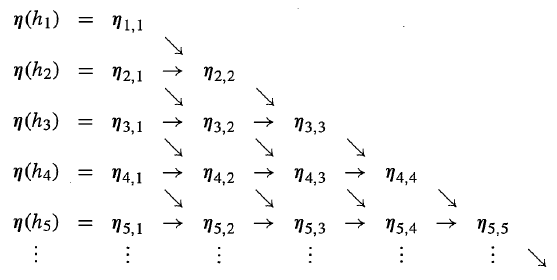
\includegraphics[scale=1]{seq.png}
\caption{Extrapolating sequence, called the Burlisch Sequence \cite{gillbook}.}
\label{fig:seq}
\end{figure}
\FloatBarrier
%
To get an idea on the error estimate, \cite{gillbook} mentions that each value $\eta_{ij}$ in column $j$ of the sequence shown in \Cref{fig:seq} provides an approximation of the true solution comparable to that provided by the \gls{RK} method of order $2j$. So when high accuracy is required, extrapolation methods definitely beat the Runge-Kutta methods.

\section{Lie Group Variational Integrator}
When it comes to simulating rigid-body dynamics such as the full two-body problem we discussed in \Cref{F2BP}, one should not use general numerical integration methods because they fail to preserve the geometric characteristics of the dynamics. For example, if we use Runge-Kutta method for numerical integration of the full two-body equation of motion, then with time the rotation matrices, say $R$, will drift from the orthonormal rotation group; the quantity $R^TR$ will drift from being an identity matrix. This means that the attitude of the rigid bodies cannot be accurately determined and since the gravitational force and moment due to the gravitational mutual potential both depend on the attitude of the rigid bodies, their computations will no longer be accurate, which will ultimately lead to a wrong two-body simulation. A solution to curb this problem is the \gls{LGVI} \cite{fahn_lgvi}.

The equations of motion presented in \Cref{F2BP} are continuous in time but \gls{LGVI} works with a discretized version of those equations. For a full derivation, the reader should refer to \cite{lee_lgvi}. The discrete time equations for the relative motion of the binary system (motion relative to one of the asteroids in the binary system) in the full two-body problem in Lagrangian form are presented as follows \cite{lee_lgvi}:
\begin{equation}
\label{lgvi1}
F_{2_n} X_{n+1} - 2X_n + F_{2_{n-1}}^T X_{n-1} = -\frac{h^2}{m} \frac{\partial U_n}{\partial X_n}
\end{equation}
%
where $X$ is the relative position of body 1 (henceforth \textbf{B1}) with respect to body 2 (henceforth \textbf{B2}); $h$ is the stepsize of integration; $U$ is the mutual gravitational potential; $m$ is the mass ratio of the two bodies defined as $\frac{m_1m_2}{m_1 + m_2}$; $F_2$ is a matrix that represents the relative attitude for \textbf{B2} between two integration steps and it ensures that the attitude matrix of \textbf{B2} i.e. $R_2$ will not drift from the orthonormal rotation group \cite{lee_lgvi}. The $F_2$ matrix is related to the rotation matrix as $F_{2_n} = R_{2_n}^T R_{2_{n+1}}$. A similar definition applies for the $F_1$ matrix as well. In the lines of relative motion a matrix $F$ is also defined such that $F = RF_1R^T$, where $R$ is the relative attitude of \textbf{B1} with respect to \textbf{B2}. The subscript $n$ denotes the integration step number.
%
\begin{equation}
\label{lgvi2}
F_{n+1} J_{dR_{n+1}} - J_{dR_{n+1}}F_{n+1}^T = F_{2_n}^T (F_n J_{dR_n} - J_{dR_n} F_n^T) F_{2_n} - h^2 S(M_{n+1})
\end{equation}
%
where $J_{dR}$ is the non-standard moment of inertia matrix for \textbf{B1} with respect to \textbf{B2} and is defined as $J_{dR} = R J_d R^T$ \cite{lee_lgvi}. The body-specific non-standard moment of inertia matrix $J_{d_i}$ where $i=1,2$ for bodies 1 and 2, is related to the standard moment of inertia matrix $J_i$ as $J_{d_i} = trace[J_{d_i}]I_{3x3} - J_{d_i}$ \cite{lee_lgvi}. $I_{3x3}$ is the identity matrix. The term $S(M)$, where M is the moment due to the gravity potential, in \Cref{lgvi2} is determined by the following relationship \cite{fahn_lgvi}:
\begin{equation}
S(M) = \frac{\partial U}{\partial R} R^T - R \frac{\partial U}{\partial R}^T
\end{equation}
%
The partial derivative of the mutual gravitational potential with respect to the relative attitude matrix has already been presented in \Cref{u_diff_T}. The notation is different but the meaning of the terms is still the same. Let's move on to the other discrete time equations used for the \gls{LGVI}:
\begin{equation}
\label{lgvi3}
F_{2_{n+1}} J_{d_2} - J_{d_2} F_{2_{n+1}}^T = F_{2_n}^T (F_{2_{n}} J_{d_2} - J_{d_2} F_{2_{n}}^T) F_{2_n} + h^2 X_{n+1} \times \frac{\partial U_{n+1}}{\partial X_{n+1}} + h^2 S(M_{n+1})
\end{equation}
%
\begin{equation}
\label{lgvi4}
R_{n+1} = F_{2_n}^T F_n R_n
\end{equation}
%
\begin{equation}
\label{lgvi5}
R_{2_{n+1}} = R_{2_n} F_{2_n}
\end{equation}
%
So \Cref{lgvi1}, \Cref{lgvi2}, \Cref{lgvi3}, \Cref{lgvi4} and \Cref{lgvi5} are effectively what are used to propagate the two-body problem. They comprise the \gls{LGVI}. Given the initial conditions $(X_0, R_0, R_{2_0}, X_1, R_1, R_{2_1})$, \Cref{lgvi4} and \Cref{lgvi5} can be used to obtain $F_0$ and $F_{2_0}$. Then \Cref{lgvi2} and \Cref{lgvi3} can be used to obtain the terms $F_1$ and $F_{2_1}$. Then the terms $X_2$, $R_2$, $R_{2_2}$ can be obtained by solving \Cref{lgvi1}, \Cref{lgvi4} and \Cref{lgvi5}. This process is then continued again and again to propagate the two-body model \cite{lee_lgvi}. This is the Lie group variational integration process which, here, has been given specifically for the two-body problem.

\section{Taylor Series Method}
\gls{TSM} has been used in the past for numerical integration of \gls{ODE} in the study of dynamical systems. \gls{TSM} has been used in the past in studies concerning Celestial Mechanics and where high-precision was required for long-term numerical simulations (see \cite{tsm2011} and references therein). \gls{TSM} has been the topic of extensive research in the field of applied mathematics. Although the theory behind this particular method for numerical integration is straight forward, its practical implementation is extremely cumbersome. In the literature, one can find several software implementations of \gls{TSM}. The list of the most important implementations is given in \cite{tsm2011}. In this section, we will particularly discuss one of the implementations (a software package written in the C programming language) \cite{taylorSoftware}, called TAYLOR, that can be used for our application. We will begin with a brief discussion on the theory of numerical integration with \gls{TSM}, following which we will briefly look into what the TAYLOR software does and how it can potentially be used for our application.

Consider the initial value problem in the following general form (where \textit{t} is the independent variable) \cite{taylorSoftware}:
\begin{equation}
    \begin{aligned}
    \dot{x}(t) &= f(t,x(t)) \\
    x(t_0) &= x_0
    \end{aligned}
\label{ivp}
\end{equation}
where \textit{f} is an analytic function in its domain of definition, $x_0$ is the initial value or the starting value of the variable $x$ corresponding to the initial time $t_0$. Given the initial condition $x(t_0) = x_0$, the value $x(t_0 + h)$ (where $h$ is the step size of integration) is approximated by the Taylor Series Expansion of the solution x(t) at $t=t_0$ \cite{taylorSoftware}:
\begin{equation}
    \begin{aligned}
    x_0 &= x(t = 0) \\
    x_{m+1} &= x_m + \dot{x}(t_m)h + \frac{\ddot{x}(t_m) h^2}{2!} + \ldots + \frac{\frac{\delta^p x(t_m)}{\delta t^p} h^p}{p!}
    \end{aligned}
\label{taylorexpansion}
\end{equation}
where $p$ is the degree of the Taylor Series expansion, $m=0, \ldots,M-1$ and $M$ is the total number of steps involved in the integration process. Note that the \gls{TSM} does not require a reduction in step size of the integrator to increase its accuracy; increasing the order of the Taylor expansion increases the integrator's accuracy \cite{taylorSoftware}. In theory, \Cref{taylorexpansion} describes how the integration is done for an \gls{ODE}. For simplicity, we will henceforth represent the $j^{th}$ derivative of the dependent variable $x$ with respect to time as $x^{(j)}(t)$. In practice, to implement \gls{TSM}, one has to compute the values of the derivatives $x^{(j)} (t_m)$ and substitute them in \Cref{taylorexpansion} to get the value of $x_{m+1}$ i.e. the integrated value of $x$. The theoretical way to achieve this is by differentiating the first expression in \Cref{ivp} with respect to time, at $t=t_m$ \cite{taylorSoftware}. This is illustrated as follows:
\begin{equation}
    \begin{aligned}
    x^1 (t_m) &= f(t_m, x(t_m)) \\
    x^2 (t_m) &= f_t(t_m, x(t_m)) + f_x(t_m, x(t_m)) x^1 (t_m)
    \end{aligned}
\end{equation}
where $f_t$ and $f_x$ are the derivatives of the function $f$ (defined in \Cref{ivp}) with respect to time and $x$ respectively. Thus, for the order $p$ of the Taylor expansion in \Cref{taylorexpansion}, the derivatives of the function $f$ (upto order $p$) have to be computed first. Then for each integration step, these derivatives have to be evaluated at $t=t_m$ to obtain the coefficients for the expansion given in \Cref{taylorexpansion} \cite{taylorSoftware}.

For the full two-body and the restricted full three-body problem that we had discussed earlier in \Cref{F2BP} and \Cref{RF3BP}, respectively, obtaining the coefficients for the Taylor expansion will be cumbersome, especially for relatively high-orders of expansion, because the differential equations of motion have a complex structure. However, there is a recursive numerical technique called \gls{AD} that allows fast computation of derivatives upto any order \cite{taylorSoftware}. The topic of \gls{AD} is quite comprehensive and as such can not be covered in this literature study. However, an explanation on \gls{AD} can be found in \cite{taylorSoftware} (also see references therein) along with a worked out example using the Van Der Pol equation. The first step in \gls{AD} technique is to decompose the function $f$ in an \gls{ODE} (see the first expression in \Cref{ivp}) into a sequence of smaller functions, which when utilizes simple algebraic operations such as addition, multiplication, subtraction, division, real powers, exponentials, logarithms and trigonometry, obtains the original function $f$ in the \gls{ODE}. The example using Van Der Pol equation in \cite{taylorSoftware} illustrates the decomposition process properly. The reason why we decompose is because \gls{AD} provides simple formulas for calculating the $n^{th}$ derivative of a function that can be decomposed into a sequence of basic operations. These formulas can also be found in \cite{taylorSoftware}, referred to as \textit{propositions} in the paper. Once the expressions for calculating the $n^{th}$ derivative of the basic functions are obtained, they can be used recursively to calculate the $n^{th}$ derivative of the function $f$ in order to get the coefficients of the Taylor expansion in \Cref{taylorexpansion}. This process is also illustrated properly in the same example as mentioned before, in \cite{taylorSoftware}. There is no general code for computing derivatives of a function using the \gls{AD} technique; instead \gls{AD} has to be coded separately for different systems \cite{taylorSoftware}. Fortunately, if we use the TAYLOR software provided by \cite{taylorSoftware}, then we do not have to code the \gls{AD} separately as the software does that internally.

The TAYLOR software, reads a set of differential equations provided by the user, decomposes them to apply \gls{AD} and then generates a $C$ code as its output that can compute all the coefficients in the Taylor expansion (see \Cref{taylorexpansion}) for a given point $(t_m, x_m)$ \cite{taylorSoftware}. So basically, the input to the software is the set of differential equations that have to be integrated (in our case, these would be the equations of motion for the two or the three-body problem) and the output of the software is a complete numerical integrator (with an option to have automatic step-size and order control) based on the \gls{TSM} \cite{taylorSoftware}. The output consists of a $C$ code and corresponding header file for the integrator. This allows the user to make a function call to the integrator from their \textit{main} code. An example on using the TAYLOR software for the \gls{R3BP} is given in \cite{taylorSoftware}. The example explains how to provide the set of differential equations to the software and the commands needed to get a compiled $C$ code for the integrator out of it.

We will now summarize the results, pertaining to the performance and applicability of TAYLOR for short and long-time simulation of the \gls{R3BP}, presented in \cite{taylorSoftware}. The accuracy of the software in a short-time simulation was tested for; the authors of \cite{taylorSoftware} called it the \textit{local error} test. For one unit of time, numerical integration of the \gls{R3BP} was performed, once using double precision and then again with extended precision (with twice the order of Taylor expansion than that used for the double precision simulation and with the same step-size). The relative error in the final position and velocity components, obtained from the two different simulations was computed and was found to be in the order of the machine precision epsilon\footnote{Machine precision epsilon is defined as the distance between 1 and the next larger floating point number}. The value for the latter was $2.22 \times 10^{-16}$ \cite{taylorSoftware}. The actual values for the errors can be found in \cite{taylorSoftware}. Note that the test results we just discussed were obtained from a short time simulation.

Similar to previous one, another simulation for longer integration time was performed. The integration was performed with both double and extended precision. During each integration run, the sequences of intersections of the orbit with the $z=0$ plane was recorded. The relative error between the results recorded from the double and extended precision simulations was calculated and plotted. As the simulation time increased, the relative error increased to an order which was five times larger than the machine precision epsilon. Another simulation, to check the preservation of the Hamiltonian of the \gls{R3BP}, with long integration time was performed. Theoretically, the Hamiltonian for the \gls{R3BP} should remain constant for a given orbit, so any drift in the initial and final value of the Hamiltonian after a long integration time can indicate the severity of error propagation in the integrator. The integration was performed with double precision with time of $10^6$ units. A drift in the initial and final value of the Hamiltonian was observed, however, \cite{taylorSoftware} considered the drift to be meaningless from a statistical point of view because the drift was relatively small compared to the length of the integration. The paper reported that for shorter integration times, the TAYLOR software could provide an integrator that is symplectic but in long term integration, biases could be observed in the Hamiltonian. The biases in the Hamiltonian over long term integration were also observed when extended precision arithmetic was used. The drift in the value of the Hamiltonian is because of truncation error (due to a finite order for the Taylor Series expansion) and round-off errors in the numerical integration process \cite{taylorSoftware}.

A comparison of the performance of \gls{TSM}, as obtained from the use of the TAYLOR software, with other commonly used integrators will be presented in \Cref{integrator_conclusion}.

\section{Performance Verification Of A Numerical Integrator}
\label{integ_verify}
Until this point we have discussed the various strategies available in the literature to numerically integrate a set of \gls{ODE}s. However, verification and validation of a numerical integrator, i.e. ensuring that the algorithms that have been implemented are correct, is more important than selecting the appropriate numerical integration scheme itself. If the algorithms have not been implemented correctly, then no matter how accurate an integration method is, the results obtained will be wrong which will eventually lead to wrong conclusions. Hence, a method must be adopted to ensure the integrity of the chosen numerical integrator.

For problems in the field of astrodynamics, a suitable method would be to integrate the unperturbed two-body problem, for both short and long integration times. Once the integration has completed, we can transform the Cartesian coordinates at each epoch into the classical orbital elements and verify that they remain conserved over extended periods of integration and for stressful cases such as highly eccentric orbits \cite{danbook}. \cite{danbook} also mentions that to verify the performance of an integrator, one can also check that the Jacobi integral (if defined for a system) remains preserved. These methods are not a proof of an integrator's accuracy but they provide effective means to verify the performance of an integrator and ensure that the algorithms have been implemented properly.

\section{Conclusion}
\label{integrator_conclusion}
The research work can be easily subdivided into two main focus areas: one is the simulation of the full two-body problem and the other is the simulation of the restricted three-body problem. For the full two-body problem, we already mentioned that the only way we can avoid a wrong simulation is by not using the general integration methods like Runge-Kutta, multistep or extrapolation. The only way one can perform an integration without violating the geometric characteristics of the two-body problem, such as drift in the attitude matrices from the orthonormal rotation group, is by using the Lie group variational integrator, for which we presented the discretized equations of motion in Lagrangian format. The approach is to simulate the entire two-body problem first using \gls{LGVI} and create a set of relevant data points consisting of position, velocity, potential, torque, moment etc. values and utilize these when we simulate the three-body problem. When we simulate the three-body problem, we do not require the \gls{LGVI} since in our case the third body is modeled as a point massless object which will not affect the dynamics of the two-body problem. Thus, there will not be any geometric characteristics to consider when it comes to simulating the orbit of the third particle around the binary system. In this regard, one can say that we can use any one of the standard integration techniques.

To compare the standard numerical integration methods for orbital computation, we will consider that an accuracy of upto 8 digits is required, which means that the position estimation will be correct upto 10 nm, which is adequate when it comes to simulating the orbit of a particle. We will compare the number of function calls that is needed to achieve this accuracy for each integration method type by evaluating the graphical results presented in \cite{integ_comp}. The graphs for Runge-Kutta, multistep, and extrapolation methods are presented as follows \cite{integ_comp}:
%
\begin{figure}[h]
\centering
\captionsetup{justification=centering}
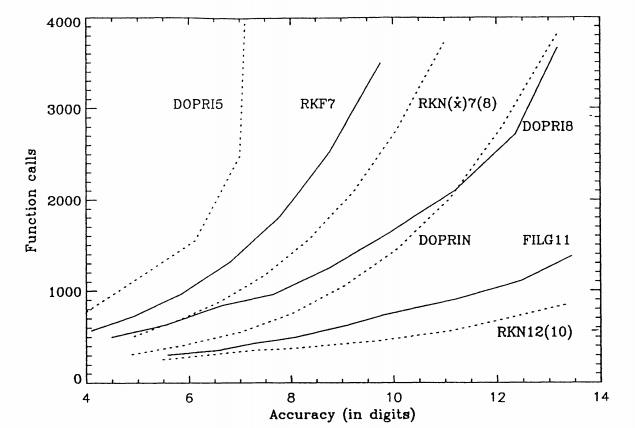
\includegraphics[scale=0.7]{rkc.png}
\caption{Function calls versus accuracy for various Runge-Kutta integrator implementations \cite{integ_comp}.}
\label{fig:rkc}
\end{figure}
\FloatBarrier
%
%
\begin{figure}[h]
\centering
\captionsetup{justification=centering}
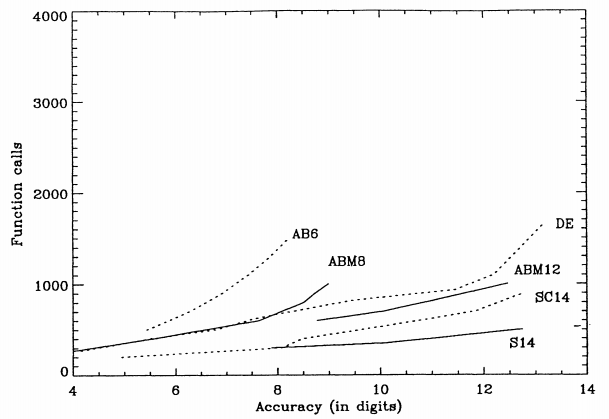
\includegraphics[scale=0.7]{multic.png}
\caption{Function calls versus accuracy for various multistep integrator implementations \cite{integ_comp}.}
\label{fig:mc}
\end{figure}
\FloatBarrier
%
%
\begin{figure}[h]
\centering
\captionsetup{justification=centering}
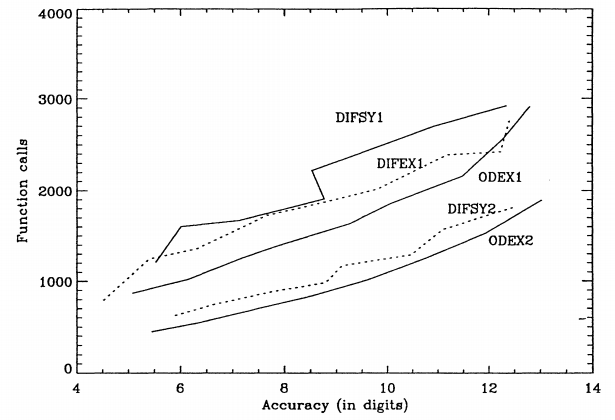
\includegraphics[scale=0.7]{exc.png}
\caption{Function calls versus accuracy for various extrapolation integrator implementations \cite{integ_comp}.}
\label{fig:exc}
\end{figure}
\FloatBarrier
%
Starting with the Runge-Kutta methods in \Cref{fig:rkc}, the methods RKN12(10), FILG11, DOPRIN are all based on Runge-Kutta Nystr\"om methods which as we discussed earlier is a method developed for the case where the acceleration term in the differential equation has no dependency on the velocity, which is not the case for the three-body problem we developed so these methods will not be utilized. The next best solution is the embedded Runge-Kutta method called DOPRI8 which is basically an $8^{th}$-order method with a $7^{th}$-order embedded method for accuracy control. For an accuracy of 8 digits, it requires a little over 1000 function calls. The coefficients for this method are readily available and the implementation of this method is the easiest of all.

Next we will consider the multistep methods in \Cref{fig:mc}. S14 and SC14 are based on Stoermer-Cowell methods which again work on differential equation forms where the acceleration does not depend on the velocity term, hence these two methods will not be considered. To get the required accuracy of 8 digits, two methods namely DE (which is a variable-stepsize and variable-order multistep Adams method) and ABM8 (which is an $8^{th}$-order Adams-Bashfort-Moulton method that utilizes the \gls{PECE} algorithm) require the same number of function calls i.e. a little less than 1000. From a computational point of view, coding the ABM8 method is much more simple than the DE method since the mathematics behind the former is much easier in comparison to that of a variable-order and stepsize method. Moreover, the coefficients for the ABM8 method are also provided in \cite{gillbook} which would drastically help in coding the algorithm in practice.

Next we will discuss the extrapolation integration methods from \Cref{fig:exc}. The methods presented here are very specific but they basically follow the same principles of extrapolation methods that we had discussed earlier. The DIFSY2 method is specially designed for differential equations that do not depend on first-order derivatives and hence this method will not be considered. The same goes for ODEX2. The remaining methods depicted in the graph provide the required accuracy for function calls way over 1000.

Finally we will discuss the \gls{TSM} for numerical integration. \cite{taylorSoftware} compares the performance of the \gls{TSM} with, and specifically their implementation, with an explicit Runge-Kutta code of order 8 and an extrapolation method of varying order based on the Gragg-Bulirsh-Stoer algorithm. \cite{taylorSoftware} notes that the \gls{TSM} and the extrapolation methods are, in general, similar to each other since both can use arbitrarily high orders. \cite{taylorSoftware} did the performance comparison by numerically solving the \gls{R3BP}, Lorenz problem and the periodically forced pendulum problem. In all the tests, the integrator produced by the TAYLOR software was superior to the other two integrators. The extrapolation method based integrator was comparable to the \gls{TSM} integrator in its performance, however, the \gls{RK} integrator performed poorly compared to the former two. Note that the integration time was small in all test cases and \cite{taylorSoftware} did not do the comparison for longer integration times.

From the application point of view, it is more important to produce reliable results rather than being concerned about the time it takes to produce highly accurate results. Of all the methods that we have discussed here, when it comes to accuracy, the extrapolation method and \gls{TSM} prove to be superior. In particular, the \gls{TSM} implementation from \cite{taylorSoftware} provides high accuracy and is also faster than its \gls{RK} and extrapolation counterparts. The \gls{TSM} from \cite{taylorSoftware} is the easiest to implement since all one has to do is to provide the differential equation in their mathematical form to the software which then automatically produces the code for the integrator. But since this integrator has not been tested for longer integration times, its reliability is questionable. We could use multistep integration methods, however they tend to be highly unstable, especially at higher-orders, unless ofcourse a \gls{PECE} algorithm is used. The latter is particularly useful for astrodynamics problems which often involve long-periods of perturbations intertwined with short-periods of intense interactions with the main body \cite{danbook}. Of all, however, the most accurate method, albeit computationally expensive, is the extrapolation method. Since we are more concerned with the accuracy than the speed of integration, extrapolation methods such as the Burlisch-Stoer algorithm offer the most superior performance and hence shall be used for the thesis.
